% Sample LaTeX file for creating a paper in the Morgan Kaufmannn two
% column, 8 1/2 by 11 inch proceedings format.

\documentclass[letterpaper]{article}
\usepackage{uai2020}
\usepackage[margin=1in]{geometry}
\usepackage{cite}
% Set the typeface to Times Roman
\usepackage{times}
\usepackage{mathtools}
\usepackage{amsmath,amssymb,amsfonts}
\usepackage{algorithmic}
\usepackage{graphicx}
\usepackage{textcomp}
\usepackage{xcolor}
\usepackage{mathtools}
\usepackage{tabu}
% \usepackage{subcaption}
\usepackage{flushend}
\usepackage{xcolor}
\usepackage[euler]{textgreek}
\usepackage{amsmath}
\usepackage{amssymb}
\usepackage{subfig}

\newdimen\imageheight
\title{Variational Inference of Infinite Generalized Gaussian Mixture Models using feature selection}

\author{} % LEAVE BLANK FOR ORIGINAL SUBMISSION.
          % UAI  reviewing is double-blind.

% The author names and affiliations should appear only in the accepted paper.
%
\author{ {\bf Srikanth Amudala} \\
Concordia Institute for \\Information Systems Engineering \\
Concordia University\\
Montreal, Canada\\srikanth.amudala@mail.concordia.ca 
\And
{\bf Nizar Bouguila}  \\
Concordia Institute for \\Information Systems Engineering \\
Concordia University\\
Montreal, Canada\\nizar.bouguila@concordia.ca
% \And
% {\bf Coauthor}   \\
% Affiliation \\
% Address    \\
% (if needed)\\
}

\begin{document}

\maketitle

\begin{abstract}
This paper presents a variational Bayesian learning
framework for the infinite generalized Gaussian mixture(IGGMM)
model. Our work is motivated with the flexibility of shape parameter in the generalized Gaussian distribution(GGD) that has proven its capability to model complex multi-dimensional
data. We also incorporate feature selection to consider the features that are most appropriate in constructing an approximate model in terms of classification and clustering accuracy. 
Experimental results on medical and image categorization dataset show the effectiveness of the proposed algorithm.
\subsection*{\textbf{Keywords}}
Data clustering, Mixture models, Variational Bayesian inference,
Generalized Gaussian Distribution, Classification, Image categorization.
\end{abstract}

\section{Introduction}
Clustering algorithms have been broadly applied in many research areas such as computer vision, signal processing, and pattern recognition. 
A mixture model, one of the most predominant statistical inference techniques,  clusters data into a collection of homogeneous groups.
Mixture models are widely incorporated for dealing with Parameter learning. 
For example, 
the most famous technique\cite{bouguila2006unsupervised} of all is the Expectation-Maximization (EM) algorithm. However, the EM algorithm also suffers from overfitting and has a high dependency on initialization\cite{stauffer1999adaptive}. 
This trade-off the efficiency of the learning algorithm and impacts the accuracy of the model.

Aside from this, an issue that normally emerges, particularly when dealing with high-dimensional 
data is the detection of the salient features. Naturally, salient features are those that encourage 
the modelling task and produce efficient outcomes. 
Uniform or unimodal features from these high dimensional data are irrelevant to clustering. Moreover, having a higer number of features may confuse the model by increasing the model complexity\cite{harrison1998organizational}\cite{law2004simultaneous}. 
This suggests that choosing the features and selecting the number of mixture components should be
addressed simultaneously.

To address both feature and model selection, we present a novel mathematical model and also by extending the Generalized Gaussian Mixture Model (GGMM) to the infinity to address the selection of the right number of mixture components. 
This reduces the computation cost and also gives a good approximation of the underlying distribution for the data.
We employ the model proposed in \cite{constantinopoulos2006bayesian}, a feature saliency determination process,
where each feature is weighted up to a probability ranging between zero and one.

This paper is organized as follows. In Section 2 we introduce the mathematical model and variational learning of the IGGMM and the experimental
results are explained in Section 3. The paper is concluded in Section 4.


\section{Mathematical Model}
The finite GGMM for a variable $\mathcal{X} \epsilon R $ with parameters mean$(\mu)$, precision$(\tau)$ and shape$(\lambda)$ is defined as follows:
\begin{equation}
    \begin{split}
        P(\mathcal{X}|\mu, \tau, \lambda) &= \frac{\lambda  \tau^\frac{1}{\lambda}}{2\Gamma(\frac{1}{\lambda})}
          e^{-\tau  |(\mathcal{X}-\mu)|^{\lambda}}    
        %   \text{where, }
        % \tau &= \Bigg({\frac{1}{\sigma} \sqrt{\frac{\Gamma(\frac{3}{\lambda})}{\Gamma(\frac{1}{\lambda})}}}\Bigg)^\lambda
    \end{split}
    \label{ggmm}
    \end{equation}
where $\tau = \bigg({\frac{1}{\sigma} \sqrt{\frac{\Gamma(\frac{3}{\lambda})}{\Gamma(\frac{1}{\lambda})}}}\bigg)^\lambda$, $\Gamma(.)$ denotes the gamma function given by $\Gamma(z) = \int_{0}^{\infty}p^{z-1}e^{-p} dp$, where $z$ and $p$ are real variables.
The shape of the probability density function is determined by the shape parameter $\lambda$.
The larger the value, the flatter the probability density function. This means that the decay rate of the density function is determined by  $\lambda$. 
Note that for the two special cases, when $\lambda = 2$ and $\lambda = 1$, the GGD is reduced to the Gaussian and the Laplacian distributions, respectively.
If $\mathcal{X}$ follows a mixture of $K$ GGDs, then 
\begin{equation}
    P(\mathcal{X}|\Theta) = \sum_{k = 1}^{K} P(\mathcal{X}|\mu_k, \tau_k, \lambda_k)\pi_k
\end{equation}


where $\pi_k(0\leq\pi_k\leq1$ and $\sum_{k=1}^{K} \pi_k = 1)$ are the mixing weights and $p(\mathcal{X}|\mu_k, \tau_k, \lambda_k)$ is the GGMM likelihood of component $k$. 
As for the symbol $\Theta = (\epsilon, \pi)$, it refers to the entire set of parameters to be estimated where $\epsilon = (\mu_1, \tau_1, \lambda_1, ..., \mu_K, \tau_K, \lambda_K)$ and $\pi=(\pi_1,...,\pi_K)$. 

Considering $N$ observations,  $\mathcal{X} = (X_1, X_2, ..., X_N)$, and supposing that the number of components $K$ is known, the data likelihood is denoted as follows:
\begin{equation}
    P(\mathcal{X}|\Theta) = \prod_{n = 1}^{N}\sum_{k=1}^{K} P({X}_n|\epsilon_k)\pi_k
\end{equation}
where $\epsilon_k = (\mu_k, \tau_k, \lambda_k)$. 
For each variable ${X}_i$, let $Z_i$  be $K$-dimensional vector known by the unobserved vector that assigns the appropriate mixture component ${X}_i$ belongs to. Then, $Z_{ik}$ is equal to 1 if ${X}_i$ belongs to class $k$ and 0, otherwise. Hence, the complete-data likelihood is given as follows:
\begin{equation}
    P(\mathcal{X}|\Theta) = \prod_{n = 1}^{N}\sum_{k=1}^{K} (P({X}_n|\epsilon_k)\pi_k)^{Z_{nk}}
\end{equation}



% The EM algorithm comprises of finding the mixture parameters that maximize the complete data log-likelihood given by:
% \begin{equation}
%     L(\mathcal{X}, Z, \Theta) = \sum_{n = 1}^{N}\sum_{k=1}^{K} Z_{nk}\ln(P(X_n|\epsilon_k)\pi_k)
% \end{equation}
% The assignment of $k^{th}$ component of the mixture can be denoted as follows\cite{b9}:
% \begin{equation}
%     \hat{Z}_{nk}^t = \frac{P^{t-1}(X_n|\epsilon_k^{t-1})p_k^{t-1}}{\sum_{k=1}^{K} P^{t-1}(X_n|\epsilon_k^{t-1}) p_k^{t-1}}
% \end{equation}
% where $t$ denotes the current step and $\epsilon_k^t$ and $p_j^t$ are the current estimates of the parameters.
% The EM algorithm produces a sequence of estimates to the mixture parameters $\Theta^t$, for $t=0,1,...,$ until a convergence measure is fulfilled through two distinctive steps: the expectation and the maximization. The EM algorithm comprises of:
% \begin{enumerate}
%     \item Initialization of the mixture parameters.
%     \item E-step: Compute $\hat{Z}^t_{nk}$ (Eq. (6)) using the initialized
%     parameters.
%     \item M-step: Update the parameters using \\
%         $\hat{\Theta}^t =$ $\argmax_{z_{\Theta}}$ $L(\Theta, Z, \mathcal{X})$.
% \end{enumerate}
% We note that the EM algorithm has some drawbacks, like convergence to local maxima due to its dependence on initialization. 
% A detailed discussion of the disadvantages of the EM algorithm is in \cite{b1}.


\subsubsection{Feature Selection}

Feature selection is an essential process in a mixture model as
some features in the data do not necessarily have importance in clustering. 
Assume $\mathcal{X}=(X_1, X_2, ..., X_N)$ is a dataset of points, each $X_N $ is a real 
factor vector in a d-dimensional space. We wish to train a mixture model by modelling this data and we expect that each mixture component density is factorized over the features. Hence, the features are considered to be independent for each mixture component. 
As we know, Not all the features might be relevant for modelling while some of the features may be more useful. Rather than expecting that there is a deterministic separation among the useful and non-useful features, 
we assume that a feature is useful up to a weight ranging from between 0 and 1. 

Thus, given a few mixture components, we assume that a feature of $\mathcal{X}$ is drawn from a mixture of two univariate subcomponents, as proposed in \cite{law2004simultaneous}. The first 
subcomponent that is distinctive for every mixture component produces necessary information, while the second subcomponent that is basic to all mixture components generates the "noisy" information.
Hence, the features follow the following distribution:

\begin{equation}
    \begin{split}
        p(X|Z, \Theta,\zeta, S) = \prod_{n=1}^N\prod_{k=1}^K\bigg[\prod_{i=1}^d p(X_i|\Theta_{ik})^{s_n} \\
        p(X|\zeta_{ik})^{1-s_n}p(S|\epsilon)\bigg]^{z_{nk}} \\
        \text{where $\Theta=\{\mu, \tau, \lambda\}$, $\zeta=\{\epsilon, \delta, \omega\}$}
    \end{split}
\end{equation}

\begin{equation}
    \begin{split}
        % p(X, Z, \pi, \mu, \tau, \lambda,S, ) = p(X|Z, \mu, \tau, \lambda) \\
        p(X, Z,& \pi, \mu, \tau, \lambda, \epsilon, \delta, \omega, S) =\\ &\prod_{n=1}^N\prod_{k=1}^K\bigg[\prod_{i=1}^d {p(X_i|Z_{nk}, \mu_{ik}, \tau_{ik}, \lambda_{ik})}^{s_i^n}\\
        &{p(X_n|Z_{nk}, \epsilon_{ik}, \delta_{ik}, \omega_{ik})}^{1-s_i^n}\bigg]
    \end{split}
\end{equation}

The model parameter mean$(\mu)$, precision$(\tau)$ and shape$(\lambda)$ of the relevant subcomponents.
Respectively, $\epsilon, \delta,$ and $\omega $ are the sets of parameters
for the irrelevant subcomponent. 
The saliency of features is expressed through the hidden variables
$s_i^n$
, where $s_i^n \in \{0, 1\}$. If the value of $s_i^n$
is one, then the $i^{th}$ feature of
$X_N$ has been generated from the relevant subcomponent; otherwise,
it has been generated from the irrelevant subcomponent.
The distribution of the 
% hidden variables $Z$ given the mixing probabilities $\pi = \{\pi_k\}$ and of the
hidden variable $S$ given the probabilities $w = \{w_i\}$ (feature
saliencies) is given as follows: 
\begin{equation}
    \begin{split}
        p(S|w) = \prod_{n=1}^N \prod_{i=1}^d w_i^{s_i^n}(1 - w_i)^{1-s_i^n}
    \end{split}
    \end{equation}
\subsection{Bayesian Learning}
% \subsection{Variational Inference of the Generalized Gaussian Mixture Model}
With in the framework of Variational Expectation-Maximization (VEM) we have proposed a variational inference approach for the GGMM \cite{b10} \cite{Bishop}.
% To achieve the closed-form updates and automatic determination of the number of mixture components by 
% optimizing the Kullback–Leibler (KL) divergence between the true posterior $p$ and the approximate distribution $q$ \cite{Bishop}.
% The smaller the KL divergence, the stronger the relationship between the distributions. The KL divergence is denoted by:
The closed-form updates and the automatic determination of the mixture components $(k)$ is obtained by optimizing the Kullback–Leibler (KL) divergence between the true posterior $p$ and the appropriate distribution $q$\cite{Bishop}. The stronger the relationship between the distribution the smaller is the KL divergence. The KL divergence is denoted by:

\begin{equation}
    \begin{split}\label{kl}
    KL(p\parallel q) & = - \int q(Z) \ln\{\frac{p(Z,\mathcal{X})}{q(Z)}-\ln p(\mathcal{X})\}dZ \\ &
    = - \int q(Z) \ln\{\frac{p(Z,\mathcal{X})}{q(Z)}\}dZ + \ln p(\mathcal{X})
    \end{split}
 \end{equation}

Calculating the evidence $\ln p(\mathcal{X})$ will give us the KL divergence. However, this is complex to calculate which motivates the proposed algorithm. 
% Reordering Eq. (\ref{kl}), we get: 
\begin{align}
    \ln p(\mathcal{X}) &= KL(p\parallel q) + \underbrace{\int q(Z) \ln\{\frac{p(Z,\mathcal{X})}{q(Z)}\}dZ}_\text{Evidence Lower Bound}\\
    \mathcal{L} &= \int q(Z) \ln\{\frac{p(Z,\mathcal{X})}{q(Z)}\}dZ
\end{align}

% \begin{equation}
%     \ln p(\mathcal{X}) = KL(p\parallel q) + \underbrace{\int q(Z) \ln\{\frac{p(Z,\mathcal{X})}{q(Z)}\}dZ}_\text{Evidence Lower Bound}
%  \end{equation}
Maximizing the Evidence Lower Bound (ELBO) is equivalent to minimizing the KL divergence. 
By applying Jensen's inequality, the ELBO serves as a lower-bound for the log-evidence, $\ln p(\mathcal{X}) \geq$ ELBO$(q)$ for any $q(Z)$, which is approximate of the posterior.  
To maximize the ELBO, we need to choose a variational family $q$.
The complexity of the family determines the flexibility in providing an appropriate approximation to the true posterior distribution.



% We assign Normal priors for the distributions mean, and Gamma
% priors for the precision and shape parameters [47,48]:
% $\mu_k \sim N(\mu| m_0, s_0^{-1}), \tau_k \sim G(\tau|\alpha_0, \beta_0), \lambda_k \sim G(\lambda|\alpha_{\lambda}, \beta_{\lambda})$ where $N(\mu| m_0, s_0^{-1})$
% is the Normal distribution with mean $m_0$ and precision $s_0^{-1}$, $G(\tau|\alpha_0, \beta_0)$
% is the Gamma distribution with shape parameter
% $\alpha_0$ and rate parameter $\beta_0$, $\lambda$, $\mu_0, s_0, \beta_0, \alpha_0$ are the 
% hyperparameters of the model.
% With these priors, the posterior distributions for $\mu, \tau, \lambda$ are defined as \cite{b9}:
% \begin{equation}
%     \begin{split}
%         p(\mu_k|Z, X) &\propto e ^{{-(\mu_k - \mu_0)^2 s_0/2} + \sum_{Z_{nk} = 1} - (\tau_k|X_n - \mu_k|)^{\lambda_k}}   \\
%         p(\tau_k|Z, X) &\propto \alpha_k ^{\alpha_0 - 1} e ^{-\beta_0 \tau_k}\tau_k^{n_j} e ^{\sum_{Z_{nk} = 1} - (\tau_k|X_n - \mu_k|)^{\lambda_k}}   \\
%         p(\lambda_k|Z, X) &\propto \lambda_k ^{\alpha_\lambda - 1} e ^{-\beta_\lambda \lambda_k}\tau_k^{n_j}\bigg(\frac{\lambda_k}{\Gamma(1/\lambda_k)}\bigg)^{n_j} \\
%         &e ^{\sum_{Z_{nk} = 1} - (\tau_k|X_n - \mu_k|)^{\lambda_k}}  
%     \end{split}
% \end{equation}
% Accordingly, we can not use the posterior distributions in their current state. 


As a result of the nonlinearity of the shape parameter, the conjugate prior distribution can not be found directly. Therefore, we considered utilizing the Taylor estimation to find an approximate lower bound of the complete data log-likelihood to determine whether an appropriate prior exists in the exponential family.


% However, the negative second-order derivative causes the function $q(\lambda)$ to be concave, resulting in an upper bound rather than a lower bound; which is required.
% Hence, we consider $\lambda$ as a parameter and it is not assigned a prior distribution\cite{b5}. 
% The conjugate exponential priors for $\mu$ and $\tau$ are Normal and Gamma distributions. Therefore, we specify all the priors according to:

\begin{figure}[h!]
    \begin{center}
        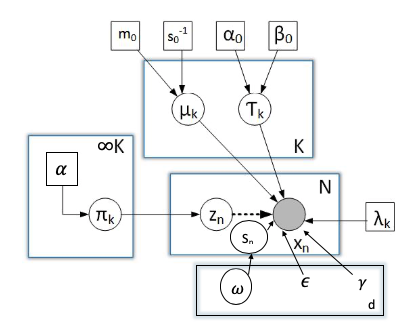
\includegraphics[width=0.7\linewidth]{pictures/graphicalmodel_v1.png}
        \caption{Graphical model for the VIGGMM with feature selection. 
        The filled circle, unfilled circles and squares represent observations, random variables, and parameters, respectively. The dependency among the variables is represented by directional arrows.}
        \label{VGGM Graphical Model}    
    \end{center}
\end{figure}

However, the second-order derivative of the function $q(\lambda)$ is negative making the function concave, resulting in an upper bound rather than a lower bound; which is required. 
Hence, $\lambda$ is considered as a parameter and is not assigned any prior distribution\cite{b5}. 
Normal and Gamma distributions are assigned as conjugate exponential priors for $\mu$ and $\tau$. This can be observed in Fig. \ref{VGGM Graphical Model} and the conjugate priors for all the model parameters are given as follows:
% \begin{equation}
%     \mu_k \sim N(\mu| m_k, s_k^{-1})   
% \end{equation}
% \begin{equation}
%     \tau_k \sim G(\tau|\alpha_k, \beta_k)    
% \end{equation}
\begin{align}
        \label{mu}
        \begin{split}
            q^\star(\mu) &= \prod_{k=1}^K\prod_{i=1}^d N(\mu_{ik}| m_{ik}, s_{ik}^{-1})   
        \end{split}\\
    \label{tau}
        \begin{split}
            q^\star(\tau) &= \prod_{k=1}^K\prod_{i=1}^d G(\tau_{ik}|\alpha_{ik}, \beta_{ik})    
        \end{split}
    \\
    \label{S}
        \begin{split}
            q^\star(S) &= \prod_{n=1}^N\prod_{i=1}^d \eta_{in}^{s_i^n}(1-\eta_{in})^{1-s_i^n}
        \end{split}
    \\
    \label{pi}
        q^\star(\pi) &=  Dir(\pi|\gamma)
    \\
    \label{gammak}
        \gamma_k &= \gamma_0 + N_k
    \\
    \label{exppi}    
    \begin{split}
        \mathop{\mathbb{E}}[\ln \pi_k] &= \psi(\gamma_k) - \psi(\hat{\gamma})
    \end{split}\\
    \label{gammak}
    \hat{\gamma} &= \sum_{k=1}^{K} \gamma_k
\end{align}
        
    

We consider a variational distribution which factorizes into the latent
variables and the parameters:
% \begin{equation}
%     q(Z, \pi, \mu, \tau, \lambda) = q(Z)q(\pi, \mu, \tau, \lambda)
% \end{equation}

\begin{equation}
    \begin{split}
        \ln q^\star(Z) = \mathop{\mathbb{E}_{\mu, \tau, \pi, s}}[\ln p(\mathcal{X}, \pi,\mu, \tau, \lambda, \epsilon, \delta, \omega, S)] + const.    
    \end{split}
\end{equation}


% \begin{equation}
%     \begin{split}
%         \ln q^\star(Z) &= \mathop{\mathbb{E_\pi}}[\ln p(Z|\pi)]+\mathop{\mathbb{E_{\mu, \tau}}}[\ln p(\mathcal{X}|Z,\mu, \tau, \lambda)]\\
%          &+ \mathop{\mathbb{E_{\mu, \tau}}}[\ln p(\mathcal{X}|Z,\mu, \tau, \lambda)]+const.
%     \end{split}
% \end{equation}

where $\mathbb{E}$ represents the expectation concerning the subscripted parameter and $const$ denotes an additive constant.
Substituting the two conditional distributions, and absorbing any terms that are independent of $Z$ into the additive constant, we have:
\begin{equation}
    \ln q^\star(Z) =  \sum_{\mathclap{n=1}}^{N} \sum_{\mathclap{k=1}}^{K}z_{nk} \ln \rho_{nk} + const
\end{equation}
where we define:
\begin{equation}
    \begin{split}\label{rownk}
        \ln \rho_{nk} = &\mathop{\mathbb{E}_{\pi}}[\ln \pi_k] + \mathop{\mathbb{E}_{\mu, \tau, s}} \bigg[\\
            &s_{nk}\bigg(\ln \frac{\lambda_k \tau_k^{\frac{1}{\lambda_k}}}{2 \Gamma (\frac{1}{\lambda_k})} - \tau_k|X - \mu_k|^{\lambda_k} \bigg)+\\
            &(1-s_{nk})\bigg(\ln \frac{\textOmega_k\Lambda_k^{\frac{1}{\delta_k}}}{2\Gamma(\frac{1}{\textOmega_k})} - 
         \Lambda_k |X_n - \delta_k|^{\textOmega_k}\bigg)\bigg]    
    \end{split}
\end{equation}
Normalizing the distribution, noting for each value of $n$ the values of $Z_{nk}$ are binary and add up to 1 overall values of $k$, we obtain:
\begin{equation}
    q^\star(Z) = \prod_{n=1}^{N}\prod_{k=1}^{K} r_{nk}^{z_{nk}}
\end{equation}
% where

The variational parameters $r_{nk}, m_{ik}, s_{ik}^{-1},\alpha_{ik}, \beta_{ik}, \eta_{in} $ are obtained by maximizing and determining the densities involved in $q$. 
The variational parameters are defined using the expected values of $z_{nk}, \mu_{ik}, s_{ik}^{-1}, s_i^n$ and functions of them. 
The following equations are obtained after deriving the expectation from $q^\star(Z),q^\star(\mu),q^\star(\tau), q^\star(S)$


% \begin{equation}
%     \mathop{\mathbb{E}}[z_{nk}] = r_{nk}
% \end{equation}
% where $r_{nk}$ denotes the responsibilities with the sum of all the responsibilities for the respective cluster $k$ given by $N_k$:

\begin{align}
    \label{rnk}
    r_{nk} &= \frac{\rho_{nk}}{\sum_{k=1}^{K}\rho_{nk}} \\
    \label{eta} 
    \eta_{in}&= \frac{w_i \hat{\eta_{in}}}{w_i\hat{\eta_{in}} + (1 - w_i)\varepsilon_{in}}\\
    \label{etain12} 
    \begin{split}
        \hat{\eta}_{in} &= \exp\bigg\{ \frac{1}{2} \sum_{k=1}^K r_{nk}[\psi(\alpha_{ik}) - \log \beta_{ik}]\\
        &-\frac{1}{2}\sum_{k=1}^{K}r_{nk} \frac{\alpha_{ki}}{\beta_{ki}}[(x_i^n - m_{ik})^2 + \tau_{ki}]\bigg\}
    \end{split}\\
     \label{epsilon}
    \varepsilon_{in} &= \exp{\bigg\{ -\frac{1}{2}\gamma_i (x_i^n - \epsilon_i)^2 + \frac{1}{2}\log\gamma_i\bigg\}}\\
    \label{Nk}
    N_k &= \sum_{\mathclap{n=1}}^{N}r_{nk}\\
    % \label{znk}
    % \mathop{\mathbb{E}}[z_{nk}] &= r_{nk} 
    % \\
    \label{mk}
    \begin{split}
        m_{ik} &= \frac{\frac{s_0m_0}{2} + t_1}
        {s_{ik}}
    \end{split}
    \\
    \label{sk}
    s_{ik} &= \frac{s_0}{2} + t_2
    % \\
    % \label{mean}
    % \begin{split}
    % \mathop{\mathbb{E}}[\ln q(\mu_k)] &= \mathop{\mathbb{E}_\tau}\bigg[\sum_{\mathclap{n=1}}^{N}(-Z_{nk}\tau_ks_n|X_n - \mu_k|^{\lambda_k}) - \\
    % &\frac{s_0}{2}(\mu_k - m_0)^2\bigg]
    % % -\frac{s_0}{2} + \sum_{\mathclap{n=1}}^{N}(r_{nk} \tau_k)\bigg]
    % \end{split}
\end{align}
% Using Binomial Expansion 
% $|X_n - \mu_k|^{\lambda_k}$ is expanded to the power 2 with the following conditions:\\
% $if(\mu_k > X_n )$
% \begin{equation}
%     \begin{split}
%         |\mu_k - X_n|^{\lambda_k}=&\mu_k^{\lambda_k} - \lambda_k \mu_k^{\lambda_k - 1} X_n +\\
%         &\frac{\lambda_k}{2} (\lambda_k - 1) \mu_k^{\lambda_k - 2} X_n^2
%     \end{split}
% \end{equation}
% $if(X_n>\mu_k)$
% \begin{equation}
%     \begin{split}
%         |X_n-\mu_k|^{\lambda_k} &= |X_n|^{\lambda_k}\bigg(1 - \frac{\mu_k}{X_n}\bigg)^{\lambda_k},\\
%         \bigg(1 - \frac{\mu_k}{X_n}\bigg)^{\lambda_k} &= 1 - \lambda_k \frac{\mu_k}{X_n} + \frac{\lambda_k}{2}(\lambda_k-1) \frac{\mu_k^2}{X_n^2}
%     \end{split}
% \end{equation}



% Substituting Eq. (29) and Eq. (30) in Eq. (28) and comparing it to the prior distribution, we obtain:
% \begin{equation}
%     \begin{split}\label{mk}
%         m_k = \frac{\frac{s_0m_0}{2} + t_1}
%         {s_k}
%     \end{split}
% \end{equation}
% \begin{equation}\label{sk}
%     s_k = \frac{s_0}{2} + t_2
% \end{equation}
where $t_1, t_2 $ have two different cases as follows:
\[
    t_1= 
\begin{cases}
    \sum_{{n=1}}^{N}(r_{nk}\bar{s}_n\bar{\tau}_{ik}\frac{\lambda_{ik}}{4}(\lambda_{ik}-1)\mu_{ik}^{\lambda_{ik}-3} x_n^2 + \\ 
        \sum_{{n=1}}^{N}(r_{nk}\bar{s}_n\bar{\tau}_{ik}\frac{\lambda_k}{2}\mu_{ik}^{\lambda_k-2}x_n))     , \text{if } X_n < m_k&\\ \\
        \sum_{n=1}^{N}r_{nk}\bar{s}_n\bar{\tau}_k\lambda_k\frac{|x_n|^{\lambda_k}}{x_n},              \text{otherwise}&
\end{cases}
\]
\[
        t_2= 
    \begin{cases}
        \sum_{{n=1}}^{N}(r_{nk}\bar{s}_n\bar{\tau}_{ik}\mu_{ik}^{\lambda_{ik}-2}),\text{if } X_n < m_{ik}&\\ \\
        \sum_{{n=1}}^{N}(r_{nk}\bar{s}_n\bar{\tau}_{ik}\frac{\lambda_{ik}}{2}(\lambda_{ik}-1)\frac{|x_n^{\lambda_{ik}}|}{x_n^2}),               \text{otherwise}
    \end{cases}
    \]


Where $\bar{\tau}$ represents $\mathop{\mathbb{E}_\tau}[\tau]$.
% Similarly, the solution for $\tau$ is as follows:
    % \begin{equation}
    %     \mathop{\mathbb{E}}[\ln q(\tau_k)] = \mathop{\mathbb{E}_\mu}\bigg[\frac{\lambda_k \tau_k^{\frac{1}{\lambda_k}}}{2\Gamma(\frac{1}{\lambda_k})} e ^ {-\tau_k |X-\mu_k|^{\lambda_k}} + \ln\tau_k^{\alpha_0 - 1} - \beta_0 \tau_k\bigg]
    % \end{equation}
\begin{align}    
    \label{alphak}
        \begin{split}
            \alpha_{ik} &= \sum_{\mathclap{n=1}}^{N} \bar{s}_n r_{nk} + \alpha_0 - 1
        \end{split}
    \\
    \label{betak}
        \beta_{ik} &= \beta_0 + \sum_{\mathclap{n=1}}^{N} \bar{s}_n r_{nk} \mathop{\mathbb{E}_\mu}[|X_n - \mu_{ik}|^{\lambda_{ik}}]
\end{align}
     \[
        \mathop{\mathbb{E}_\mu}[|X_n - \mu_{ik}|^{\lambda_{ik}}]=\\
    \begin{cases}
         |X_n|^{\lambda_{ik}} - \lambda_{ik} \frac{|X_n|^{\lambda_{ik}}}{X_n} m_{ik} + \\
            \frac{\lambda_{ik}(\lambda_{ik} - 1)}{2} \frac{|X_n|^{\lambda_{ik}}}{X_n^2}(\frac{1}{s_{ik}} + m_{ik}^2)     , \\\text{if } X_n > \mu_{ik}&\\ \\
            \mathop{\mathbb{E}}[|\mu_{ik}|^{\lambda_{ik}} - \lambda_{ik} \mu_v^{\lambda_{ik} - 1} X_n + \\ 
            \frac{\lambda_{ik}}{2} (\lambda_{ik} - 1) \mu_{ik}^{\lambda_{ik} - 2} X_n^2],              \text{otherwise}&
        \end{cases}
    \]    
    \text{Then using confluent hypergeometric function:}
    \begin{equation}
        \begin{split}
            \displaystyle \operatorname {\mathbb{E}} \left[|\mu_{ik}|^{\lambda_{ik}}\right]&=\\
            (\frac{1}{\sqrt{s_{ik}}})^{\lambda_{ik}}\cdot 2^{\lambda_{ik}/2}&{\frac {\Gamma \left({\frac {1+\lambda_{ik}}{2}}\right)}{\sqrt {\pi }}}
            {}_{1}F_{1}\left(-{\frac {\lambda_{ik}}{2}},{\frac {1}{2}},-{\frac {1}{2}}\left({m_{ik}}\right)^{2} s_{ik} \right).  
        \end{split}
    \end{equation}
After the maximization of Lowerbound $\mathcal{L}$ with respect to $Q$, the second step
of the method requires maximization of $\mathcal{L}$ with respect to $\pi_k$, $w_i$, $\epsilon_i$,
and $\gamma_i$. Setting the derivative of $\mathcal{L}$ with respect to the parameters
equal to zero\cite{constantinopoulos2006bayesian}, we get the following update rules:
\begin{align}
    \label{pik}
    \pi_k &= \frac{1}{N}\sum_{n=1}^N r_{nk}
    \\
    \label{wi}
    w_i &= \frac{1}{N}\sum_{n=1}^N\eta_{in}
    \\
    \label{epsiloni}
    \epsilon_i &= \frac{\sum_{n=1}^N \eta_{in}x_i^n}{\sum_{n=1}^N\eta_{in}}
    \\
    \label{gammai}
    \frac{1}{\gamma_i} &= \frac{\sum_{n=1}^N \eta_{in}(x_i^n-\epsilon_i)^2}{\sum_{n=1}^N\eta_{in}}
\end{align}
        Given the posterior distributions from the VE-step, the VM-step updates the parameters by maximizing the approximate lower bound $\mathcal{L}$.
        To estimate the parameters of the GGMM (i.e. $\lambda$), 
        \begin{equation}
            \begin{split}\label{lambda}
                \lambda_k^\star = \lambda_k + s \Delta \lambda_k   \\
                \text{where }
                \Delta\lambda_k = - \frac{\mathcal{L}^{'}_k(q, \Theta)}{\mathcal{L}^{''}_k(q, \Theta)}
            \end{split}
        \end{equation}
        where $s$ is determined by the backtracking line search \cite{b6}. 
        \subsection{Infinite Mixture Model}
        The mixing weights, $\pi_k$, are considerded to be a symmetric Dirichlet prior with concentration parameter $\alpha/k$
        \begin{align}
                \label{z given pi}
                p(Z|\pi)&= \prod_{k=1}^{K}\pi_k^{n_k}
            \\
            \label{pi dirchlet}
            \begin{split}
                p(\pi|\alpha)&\sim Dirichlet\bigg(\frac{\alpha}{K},..,\frac{\alpha}{K}\bigg) \\
                &= \frac{\Gamma(\alpha)}{\Gamma(\frac{\alpha}{K})^K} \prod_{k=1}^K\pi_k^{\frac{\alpha}{K}-1}
            \end{split}
    \end{align}
        Using the standard Dirichlet integral, we can integrate the mixing weights and the prior can be directly written in terms of indicators.
        \begin{equation}
            \begin{split}
                p(Z|\alpha) =& \int p(Z|\pi) p(\pi|\alpha)d\pi \\
                =&\frac{\Gamma(\alpha)}{\Gamma(N+\alpha)} \prod_{k=1}^K \frac{\Gamma(\frac{\alpha}{K}+n_k)}{\Gamma(\frac{\alpha}{K})}
            \end{split}
            \label{indicator_int}
        \end{equation}
        
        The conditional prior for the single indicator from
        Eq. \ref{indicator_int} by keeping all but a single indicator fixed:
        \begin{equation}
            \begin{split}
                p(Z_{nk} = 1|\alpha, Z_{-n}) = \frac{n_{-nk} + \alpha/K}{N -1 +\alpha}
            \end{split}
            \label{indicator}
        \end{equation}
        
        where the subscript $-n$ indicates all indexes except $n$ and $n_{-nk}$ is the number of observations,
        excluding $X_i$, that are associated with component $k$.
        
        
        So far, we considered the number of mixtures $K$ as a fixed finite quantity, 
        we will extend the model by updating the posteriors in Eq. \ref{indicator} with $K\rightarrow \infty$
        \begin{equation}
            p(Z_{nk} = 1|\alpha, Z_{-n})= 
            \begin{cases}
                \frac{n_{-nk}}{N -1 +\alpha} \text{     if     } n_{-nk}>0\\ 
                \frac{\alpha}{N -1 +\alpha} \text{     if     } n_{-nk}=0
            \end{cases}
            \label{indicator_cases}
        \end{equation}
        
        where $n_{nk}>0$ occurs when mixture $k$ is represented. A sample
        $X_i$ is associated with an existing component by a certain probability
        proportional to the number of samples already allocated to this component;
        while an unrepresented mixture component is proportional to $\alpha$ and $N$.
        We combine the likelihood from Eq. \ref{ggmm} on the indicators with the prior from
        Eq. \ref{indicator_cases} to obtain the conditional posteriors for the indicators
        \begin{equation}
            \begin{split}
                p(Z_{nk} = 1| ...)= \\
                \begin{cases}
                    \frac{n_{-nk}}{N -1 +\alpha}p(\mathcal{X}|\Theta) &\text{     if     } n_{-nk}>0\\ 
                    \frac{\alpha}{N -1 +\alpha}\int p(\mathcal{X}|\Theta) p(\Theta|\mu, \tau)d\Theta &\text{     if     } n_{-nk}=0
                \end{cases}    
            \end{split}
            \label{indicator_cases}
        \end{equation}
        
        Our complete algorithm can then be summarized as follows:         
\subsection*{\textbf{Algorithm}}
\begin{enumerate}
    \item Initialize the parameters and the assignments.
    \item \textbf{loop}
    \item Update mixture parameters $\mu_k, \tau_k, S,\lambda_k$ from the posteriors in Eq. \ref{mu}, Eq. \ref{tau}, Eq. \ref{S} and Eq. \ref{lambda}
    \item Update hyperparameters $m_k, s_k, \alpha_{ik}, \beta_{ik} ,\eta_{in} $ and Dirichlet process concentration parameter $\alpha$ from Eq. \ref{eta} to Eq. \ref{lambda}
    \item Update the indicators conditioned on the other indicators and the hyperparameters from Eq. \ref{indicator_cases}
    \item The convergence criteria is reached when the difference of the current value of
    joint posteriors and the previous value is less than $1e-9$. Otherwise, repeat above
    loop until convergence
    \item \textbf{end}
\end{enumerate}
\section{Experimental results and discussion}
We evaluate the built variational IGGMM (VIGGMM) using two different datasets focused on
image categorization and binary classification. We compare the effectiveness of the
model based on Gaussian mixutre model (GMM) and Variational Gaussian mixture model (VGMM).
% \subsection{Implementation details}
\subsection{Image categorization}


Image categorization and determining patterns in terms of automation plays an important role in multimedia applications \cite{maanicshah2019variational}. 
For our application, we choose the Caltech 101 \cite{fei2004learning} objects dataset.
Among the 101 categories, we chose four categories: Bikes, Yin Yang, Sunflowers, Aeroplanes. All the categories have 60 images each to have a balanced dataset. 
Sample images of these categories are shown in Fig. \ref{figure1}. 
Also, to evaluate the robustness of our model, all the categories that are considered have a similar landscape. 
\begin{figure}[h!]
    \subfloat[Bike]{%
    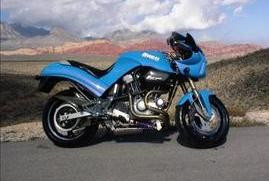
\includegraphics[height=0.1\textheight]{pictures/bike4.jpg}}
    \hspace*{\fill}
    \subfloat[Yin Yang]{%
    
\includegraphics[height=0.1\textheight]{pictures/yinyang1.jpg}}


    \subfloat[Sunflower]{%
    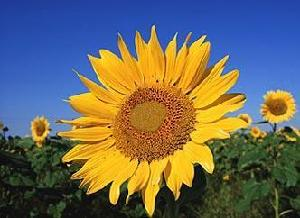
\includegraphics[height=0.1\textheight]{pictures/sunflower2.jpg}}
    \subfloat[Aeroplan]{%
    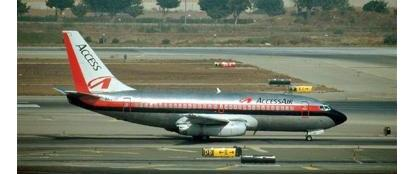
\includegraphics[height=0.1\textheight]{pictures/image_0723.jpg}}

\caption{Sample images from different categories of Caltech 101 dataset}
    \label{figure1}
\end{figure}

To implement our model on the images we need to initially create a bag of visual words model \cite{li2010contextual}\cite{csurka2004visual}. 
To create a bag of visual words model, we need to initially extract some kind of descriptors from the images. The most commonly utilized descriptors are SIFT \cite{lowe2004distinctive}, 
SURF \cite{bay2008speeded}, HOG \cite{dalal2005histograms}, and so forth. For our situation we found the SIFT 
descriptors to be an effective choice. Consequently, we first extract 
the SIFT features from the images and perform K-means 
clustering over the extracted SIFT descriptors to form the bag of the words feature vector for each image. This is utilized as input to our model. 
Table \ref{confusion Caltech} and Table \ref{classificationo report Caltech 101} shows the confusion matrix and the classification report of the VIGGMM by considering 200 features from the bag of words feature vector. 
Table \ref{features 200 Caltech} shows the performance of our model by comparing to the other
models.
We can observe that the precision and accuracy of the class Aeroplan is less than the other classes due to the very high similarity of the images.

We can see that our model VIGGMM with feature selection has performed better than all the other models. Table \ref{features 300 Caltech} shows similar results when we considered using 300 features from the bag of words feature vector.





\begin{table}
    \caption{Confusion matrix of VIGGMM for Caltech 101 dataset }
    \label{confusion Caltech}
    \centering
    \resizebox{\columnwidth}{!}
    {%
    \begin{tabular}{lllll}
        \multicolumn{1}{c}{\bf }  &\multicolumn{1}{c}{\bf Yin Yang}&\multicolumn{1}{c}{\bf Aeroplan}&\multicolumn{1}{c}{\bf Bike} &\multicolumn{1}{c}{\bf Sunflower}   \\
        \hline \\
        Yin Yang         &\textbf{5} &1&0&1 \\
        Aeroplan             &1  &\textbf{4}&0&0\\
        Bike             &0  &3&\textbf{3}&0\\
        Sunflower             &0  &0&0&\textbf{6}\\
        % 4             &Cell body (contains cell nucleus) &Output terminal &Output terminal &Output terminal &Output terminal\\
        \end{tabular}
    }
\end{table}


\begin{table}
    \caption{Classification report of VIGGMM for Caltech 101 dataset}
    \label{classificationo report caltech 101}
    \centering
    \resizebox{\columnwidth}{!}
    {%
    \begin{tabular}{lllll}
        \multicolumn{1}{c}{\bf }  &\multicolumn{1}{c}{\bf precision}&\multicolumn{1}{c}{\bf recall}&\multicolumn{1}{c}{\bf f1-score} &\multicolumn{1}{c}{\bf support}   \\
        \hline \\
        Yin Yang         &0.83 &0.71&0.77&7 \\
        Aeroplan             &0.50  &0.80&0.62&5\\
        Bike             &1.00  &0.50&0.67&6\\
        Sunflower             &0.86  &1&0.92&6\\\\
        micro avg             &0.75  &0.75&0.75&24\\
        macro avg             &0.86  &0.75&0.74&24\\
        weighted avg             &0.86  &0.75&0.75&24\\
        % 4             &Cell body (contains cell nucleus) &Output terminal &Output terminal &Output terminal &Output terminal\\
        \end{tabular}
    }
\end{table}

\begin{table}[h]
    \caption{Accuracy of different models for Caltech 101 dataset with 200 features}
    \label{features 200 Caltech}
    \begin{center}
    \begin{tabular}{lllll}
    \multicolumn{1}{c}{\bf Method}  &\multicolumn{1}{c}{\bf Features} &\multicolumn{1}{c}{\bf Accuracy($\%$)}   \\
    \hline \\
    GMM         &200 &33 \\
    VGMM             &200  &23\\
    VIGGMM             &200  &74\\
    % 4             &Cell body (contains cell nucleus) &Output terminal &Output terminal &Output terminal &Output terminal\\
    \end{tabular}
    \end{center}
\end{table}

\begin{table}[h]
    \caption{Accuracy of different models for Caltech 101 dataset with 300 features}
    \label{features 300 Caltech}
    \begin{center}
    \begin{tabular}{lllll}
    \multicolumn{1}{c}{\bf Method}  &\multicolumn{1}{c}{\bf Features} &\multicolumn{1}{c}{\bf Accuracy($\%$)}   \\
    \hline \\
    GMM         &300 &24 \\
    VGMM             &300  &23\\
    VIGGMM             &300  &72\\
    % 4             &Cell body (contains cell nucleus) &Output terminal &Output terminal &Output terminal &Output terminal\\
    \end{tabular}
    \end{center}
    \end{table}


\subsection{Binary Classification}
To verify the performance of our model in binary classification situation, we choose just the Bikes and the Aeroplan images from the Caltech 101 dataset which has an almost similar landscape. 
Table \ref{confusion caltech binary} and Table \ref{classification report caltech binary} shows the confusion matrix and classification report of our model. 
Table \ref{binary classification Caltech 101} shows the performance of our model by considering 200 features from the bag of words feature vector and compared to the other
models. 

We also applied our VIGGMM estimation algorithm in medical applications involving
detection of heart diseases\footnote{https://www.kaggle.com/ronitf/heart-disease-uci.}. 
The heart disease data set provides all the potential symptoms of a person with positive heart disease. 
This database contains 76 attributes, but all distributed tests refer to employing a subset of 14. The objective field alludes to the presence of heart infection within the patient.
Fig. \ref{histogram of Heart Disease data} shows the histogram of the heart disease dataset for all the features. 


\begin{figure}[h!]
    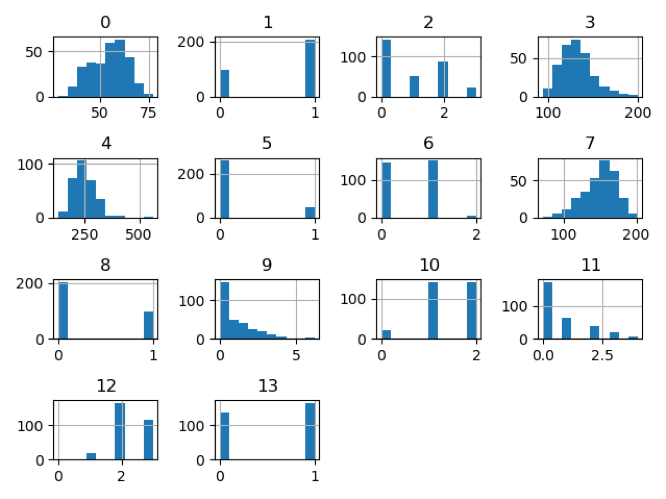
\includegraphics[width=\linewidth]{pictures/heart.png}
    \caption{Histograms of Heart Disease. Histogram-0 to Histogram-12 represent the features, Histogram-13 represents the target value.
    X-axis represents the value range and y-axis represents the frequency.}
    \label{histogram of Heart Disease data}
\end{figure}

\begin{table}[h]
    \caption{Confusion matrix of VIGGMM for Caltech 101 dataset}
    \label{confusion caltech binary}
    \begin{center}
        \begin{tabular}{lllll}
            \multicolumn{1}{c}{\bf }  &\multicolumn{1}{c}{\bf Aeroplan}&\multicolumn{1}{c}{\bf Bike}   \\
            \hline \\
            Aeroplan          &\textbf{68} &6\\
            Bike             &10  &\textbf{76}\\
            
            % 4             &Cell body (contains cell nucleus) &Output terminal &Output terminal &Output terminal &Output terminal\\
            \end{tabular}
        
    \end{center}
    \end{table}
    \begin{table}
        \caption{Classification report of VIGGMM for Caltech 101 dataset}
        \label{classification report  caltech binary}
        \centering
        \resizebox{\columnwidth}{!}
        {%
        \begin{tabular}{lllll}
            \multicolumn{1}{c}{\bf }  &\multicolumn{1}{c}{\bf precision}&\multicolumn{1}{c}{\bf recall}&\multicolumn{1}{c}{\bf f1-score} &\multicolumn{1}{c}{\bf support}   \\
            \hline \\
            Aeroplan          &0.87 &0.92&0.89&74 \\
            Bike              &0.93  &0.88&0.90&86\\\\
            
            micro avg             &0.90  &0.90&0.90&160\\
            macro avg             &0.90  &0.90&0.90&160\\
            weighted avg             &0.90  &0.90&0.90&160\\
            % 4             &Cell body (contains cell nucleus) &Output terminal &Output terminal &Output terminal &Output terminal\\
            \end{tabular}
        }
    \end{table}

        
    \begin{table}[h]
        \caption{Accuracy of different models for binary classification using Caltech 101 dataset}
        \label{binary classification Caltech 101}
        \begin{center}
        \begin{tabular}{lllll}
        \multicolumn{1}{c}{\bf Method}  &\multicolumn{1}{c}{\bf Features} &\multicolumn{1}{c}{\bf Accuracy($\%$)}   \\
        \hline \\
        GMM         &200 &60 \\
        VGMM             &200  &68\\
        VIGGMM             &200  &92\\
        % 4             &Cell body (contains cell nucleus) &Output terminal &Output terminal &Output terminal &Output terminal\\
        \end{tabular}
        \end{center}
    \end{table}


\begin{table}
    \caption{Classification report of VIGGMM for Heart disease dataset}
    \label{classification report  Heart disease}
    \centering
    \resizebox{\columnwidth}{!}
    {%
    \begin{tabular}{lllll}
        \multicolumn{1}{c}{\bf }  &\multicolumn{1}{c}{\bf precision}&\multicolumn{1}{c}{\bf recall}&\multicolumn{1}{c}{\bf f1-score} &\multicolumn{1}{c}{\bf support}   \\
        \hline \\
        Negative          &0.79 &0.76&0.78&34 \\
        Positive              &0.81  &0.83&0.82&41\\\\
        
        micro avg             &0.80  &0.80&0.80&75\\
        macro avg             &0.80  &0.80&0.80&75\\
        weighted avg             &0.80  &0.80&0.80&75\\
        % 4             &Cell body (contains cell nucleus) &Output terminal &Output terminal &Output terminal &Output terminal\\
        \end{tabular}
    }
\end{table}
        \begin{table}
            \caption{Confusion matrix of VIGGMM for Heart disease dataset }
            \label{confusion heart disease}
            \centering
            \resizebox{\columnwidth}{!}
            {%
            \begin{tabular}{lllll}
                \multicolumn{1}{c}{\bf }  &\multicolumn{1}{c}{\bf Positive Heart Disease}&\multicolumn{1}{c}{\bf Negative Heart disease}   \\
                \hline \\
                Positive          &\textbf{26} &8\\
                Negative             &7  &\textbf{34}\\
                
                % 4             &Cell body (contains cell nucleus) &Output terminal &Output terminal &Output terminal &Output terminal\\
                \end{tabular}
            }
        \end{table}

        \begin{table}[h]
            \caption{Accuracy of different models for binary classification using Heart Disease UCI dataset}
            \label{binary classification heart Disease}
            \begin{center}
            \begin{tabular}{lllll}
            \multicolumn{1}{c}{\bf Method}  &\multicolumn{1}{c}{\bf Features} &\multicolumn{1}{c}{\bf Accuracy($\%$)}   \\
            \hline \\
            GMM         &13 &50 \\
            VGMM             &13  &57\\
            VIGGMM             &13  &76\\
            % 4             &Cell body (contains cell nucleus) &Output terminal &Output terminal &Output terminal &Output terminal\\
            \end{tabular}
            \end{center}
            \end{table}
We have implemented our VIGGMM classifier using cross-validation with the split size of 4. 
The label for each data point is determined with the largest component among the likelihood of the data point belonging to the classes.
Table \ref{classification report  Heart disease}  and Table \ref{confusion heart disease} shows the confusion matrix and the classification report of the VIGGMM. 
Table \ref{binary classification heart Disease} presents the model accuracy in comparison with Gaussian Mixture Model(GMM), Variational Gaussian Mixture Model(VGMM). We can see that the VIGGMM performed better than all the other models.
            
\section{Conclusion}
We have presented a variational inference approach for IGGMM with feature selection by 
considering the shape parameter as a variable and using Binomial Expansion, 
we estimate the expectation of the distributions. Hence, the posterior distributions 
of the inference can be updated by the corresponding hyperparameters.
In the VM-step, the shape parameter is updated using the single-step update of Newton’s method. 
Also, we address the challenges of parameter learning and choosing the correct number of 
mixture components by introducing Bayesian learning and extension of the 
GGMM model to infinity.

Experimental results show that the VIGGMM with feature selection is an accurate model for image categorization and medical applications by effectively estimating the parameters.
Moreover, our model outperformed Gaussian and variational Gaussian mixture models which are known to be industry standards.  



% \newpage

% \subsubsection*{Acknowledgements}

% Use unnumbered third-level headings for the acknowledgements title.
% All acknowledgements go at the end of the paper.


% \subsubsection*{References}

% References follow the acknowledgements.  Use unnumbered third level
% heading for the references title.  Any choice of citation style is
% acceptable as long as you are consistent.


% J.~Alspector, B.~Gupta, and R.~B.~Allen  (1989). Performance of a
% stochastic learning microchip.  In D. S. Touretzky (ed.), {\it Advances
% in Neural Information Processing Systems 1}, 748-760.  San Mateo, Calif.:
% Morgan Kaufmann.

% F.~Rosenblatt (1962). {\it Principles of Neurodynamics.} Washington,
% D.C.: Spartan Books.

% G.~Tesauro (1989). Neurogammon wins computer Olympiad.  {\it Neural
% Computation} {\bf 1}(3):321-323.
\bibliographystyle{IEEEtran}
\bibliography{ref}
\end{document}
